\begin{table}[htb]
    \renewcommand{\arraystretch}{1.5}
    \begin{tabular*}{\textwidth}{|>{\columncolor{orange!15}}p{3cm}|p{17.3cm}|}
    \textbf{\large Finding} & \textbf{\large Insecure coding leads to disk-image access}\section*{}\addcontentsline{toc}{section}{Finding 9 - Insecure coding leads to disk-image access}\label{chap:Insecure}
    \\
    Risk& Medium\\
    Category& Obfuscation, information disclosure\\
    Impact& An attacker can obtain the passphrase to decrypt the disk-image file 'container.img'\\\\ 
    Description& Analyzing the file system of the server named 'plunder' running on port 22, a disk-image file 'container.img' was found. After trying to mount the image the following error message appeared:
    \newline
    \newline
    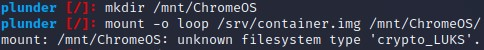
\includegraphics{mount_error.jpg}
    \newline
    \newline
    Given that the filesystem is apparently from type 'crypto\_LUKS' the disk-image is most likely encrypted. Through research the following command was tried to decrypt the filesystem:
    \newline
    \newline
    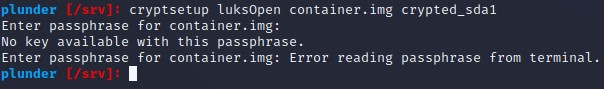
\includegraphics{cryptsetup_enterpassphrase.jpg}
    \newline
    \newline
    The first method to access the container image was a brute force attack. Since we have credentials for the SSH we copied the image to our local kali linux machine with the following command: ''scp root@172.16.0.29:/srv/container.img output.img''
    After copying the file a brute force attack was performed using the tool bruteforce-luks.
    \newline
    \newline
    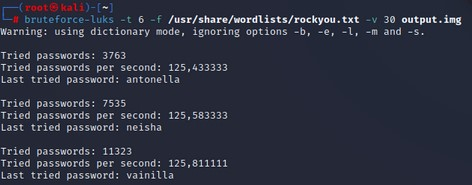
\includegraphics{brute-force-luks.jpg}
    \newline
    \newline
    However there was no matching password found with this method.   
    \\\\\\\\\\\\\\\\\\\\\\\\\\\\\\
    \end{tabular*}
    \end{table}
    \newpage
    \begin{table}[htb]
        \renewcommand{\arraystretch}{1.5}
        \begin{tabular*}{\textwidth}{|>{\columncolor{orange!15}}p{3cm}|p{17.2cm}|}
        \textbf{\large Finding} & \textbf{\large Insecure coding leads to disk-image access}\\
        
        &\\
        Description& By analyzing the processes of the server we found that a compiled python file 'fdesetup.pyc' is executed directly after rebooting the server. Unfortunately it is not possible to read a compiled python file without decompiling it. The contents of the 'fdesetup.pyc' file appear as follows:
        \newline
        \newline
        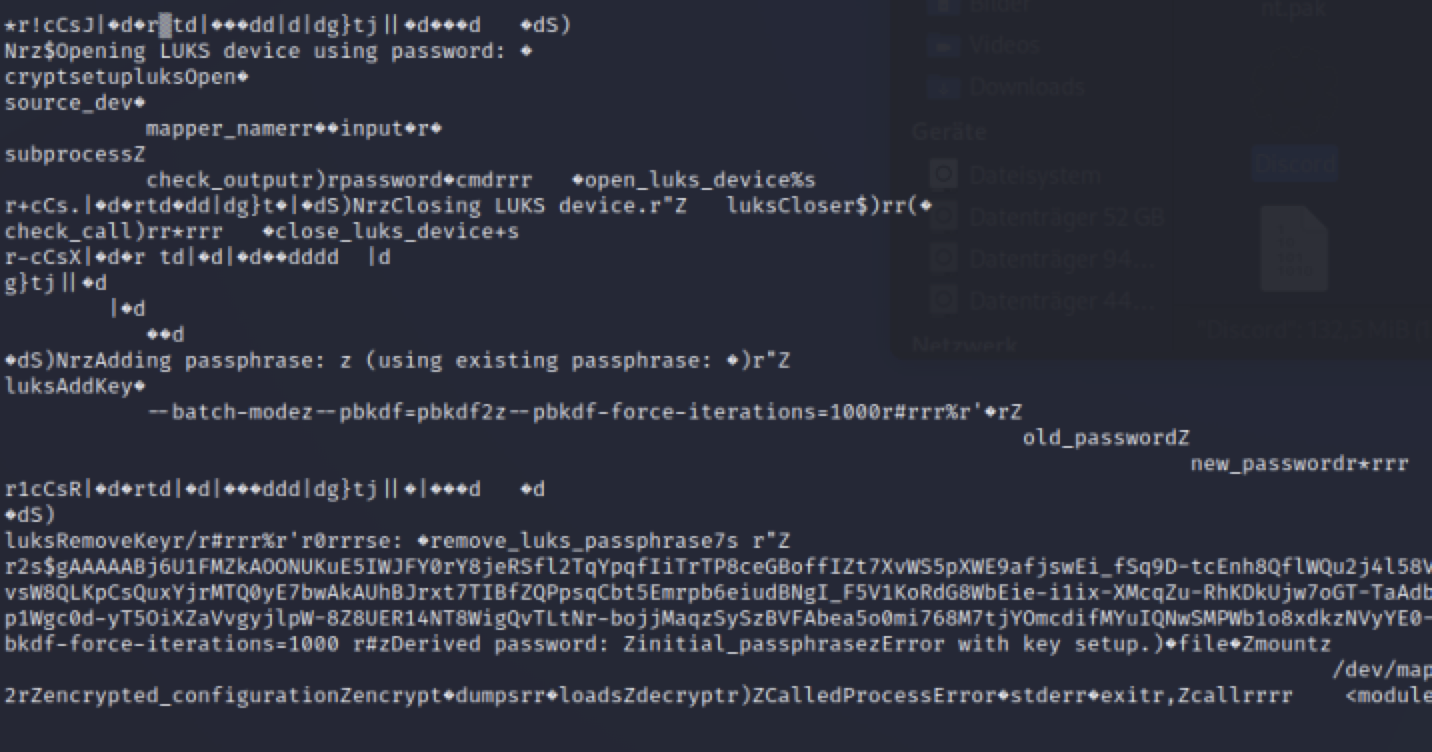
\includegraphics[width=0.73\textwidth]{fdesetup_pyc.png}
        \newline 
        \newline
        The few readable keywords inside the file like 'passphrase' or 'cryptsetupluksOpen' indicate that it must be a configuration for the 'cryptsetup luks' libary. 
        Therefore the file was copied to the local kali machine to decompile it. Since the tool 'decompyle6' didn't work for this specific file a script was written to decompilation:
        \newline
        \newline
        \begin{lstlisting}[language=python]
    GNU nano 6.4
    import dis
    def extract_code_from_pyc_file(pyc_file_path): 
        with open(pyc_file_path, 'rb') as f:
            magic = f.read(4)
            moddate = f.read(4)
            code = f.read()
        if magic b'\x03\xf3\r\n' and magic # b'\x03\xf3\r\r':
            raise ValueError("Invalid .pyc file magic: %s" % repr(magic))
        return dis.disassemble(code)
    extract_code_from_pyc_file(/home/kali/Schreibtisch/todecompile.pyc)
        \end{lstlisting}
        \\
        &However this script failed to open this file as well.    
    \\\\\\\\\\\\\\\\\\\\
    \end{tabular*}
        \end{table}
\newpage
\begin{table}[htb]
    \renewcommand{\arraystretch}{1.5}
    \begin{tabular*}{\textwidth}{|>{\columncolor{orange!15}}p{3cm}|p{17.2cm}|}
    \textbf{\large Finding} & \textbf{\large Insecure coding leads to disk-image access}\\
    
	&\\
	Description& After researching several methods the tool 'pycdc' worked for this specific file. Inside the decompiled file an encrypted configuration was found (see attachment \ref{sec:attachment1}). Luckily the file included the private key to decrypt the configuration. The cipher used is fernet. The following script decrypted the encrypted configuration:

    \begin{lstlisting}[language=python]
#! /usr/bin/python
from cryptography.fernet import Fernet
key = b'dGH1BR5gJ6wz6rneOkvmW50UsgY_J3kBZlRIUmsSiYw='

f = Fernet(key)

token=b'gAAAAAB6U1FZADONUKESIJFYDrY8jeRSFL2TqYpqfIiTrTP8ceGBoffIZt7X
vWS5pXWE9afjswEi_fSq9D-tcEnh8QflWQu2j4158VrbjbD1s8kWRqcv665XHDiFSED
PAL1yb2w=='

decrypted f.decrypt(token)

print(decrypted)


\end{lstlisting}
    The output of the script is: 
    \begin{lstlisting}[language=python]
b'{"debug": false "initial_passphrase":"Q99mjPp4xMwnEpgJd4kd5LNe",
"mapper_name": "fde", "source_dev": "/srv/container.img",
"interface_mac": "eth0", "source_files": [["/proc/cpuinfo",  "filter_cpuinfo"],  ["/sys/kernel/debug/bluetooth/hci0/identity",  null], ["/sys/devices/platform/soc/3f980000.usb/usb1/1-1/1-1.1 /1-1.1
:1.0/net/eth0/address", null]]}'
\end{lstlisting}

From the output it can be extracted that ''debug'' is set to ''false''. By examining the decompiled file we found out that the passphrase of the container image gets printed when ''debug'' is set to ''true''. Owning the key of the fernet encryption it was possible to encrypt the same configuration we just decrypted while setting ''debug'' to ''true'' instead of ''false''. The tool vim now enables the exchange of the old encrypted configuration with the new one while the debug mode is set to true and still maintains the magic bytes of the compiled python file. After those changes the file was executed and had the following output including the passphrase of the encrypted container:
\newline
\newline
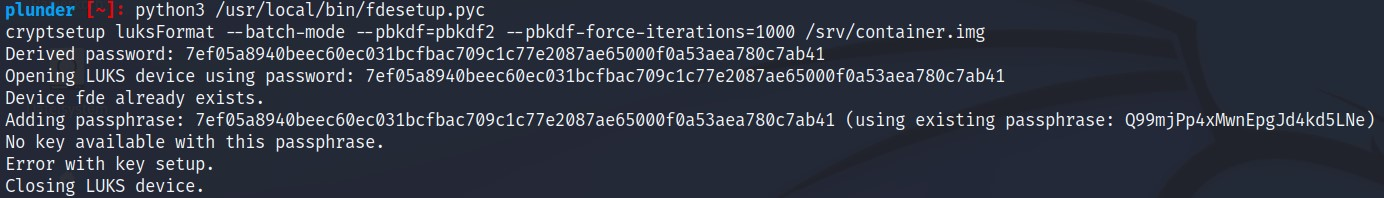
\includegraphics[width=0.85\textwidth]{passphrase.jpg}
\newline
\newline
With the given output from above we were able to access the container image.
\\\\\\\\\\\\\\\\\\\\\\\\\\
    \end{tabular*}
    \end{table}

\newpage

\begin{table}[htb]
    \renewcommand{\arraystretch}{1.5}
    \begin{tabular*}{\textwidth}{|>{\columncolor{orange!15}}p{3cm}|p{17.2cm}|}
    \textbf{\large Finding} & \textbf{\large Insecure coding leads to disk-image access}\\
    Description&
    Nevertheless no content was visible for because the device had to be mounted first. The following command made this happen: 
    \newline
    \newline
    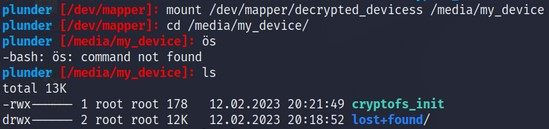
\includegraphics{mounted.jpg}
	\\ 
	&\\
	&\\
    Recommendation& The encryption process of the configuration should be outsourced in a different file and the fernet key shouldn't be displayed in plain text. Further it should't be possible for an attacker to change the current configuration and execute the file again. Additionally the debug mode should not print the whole passphrase of the container. Therefore a message could be printed which tells the user that a passphrase is used but not which one.\\    
    \\\\\\\\\\\\\\\\\\\\\\\\\\\\\\\\\\\\\\\\\\\\\\\\\\\\
    \end{tabular*}
    \end{table}